\documentclass[12pt]{beamer}


\mode<presentation>{
	\usetheme{Copenhagen}
	
	\usecolortheme[RGB={0, 0, 102}]{structure}
	  % or ...
	
	  %\setbeamercovered{transparent}
	  % or whatever (possibly just delete it)
	  
	%\usecolortheme{albatross}
	%\usecolortheme{lily}
	
	\useinnertheme{rectangles}
	\useoutertheme{smoothbars}
	\usefonttheme{structurebold}
}

\definecolor{HuskyPurple}{RGB}{57, 39, 91}
\definecolor{HuskyGold}{RGB}{226, 210, 163}
\definecolor{CalBlue}{RGB}{0, 0, 102}
\definecolor{CalGold}{RGB}{255, 204, 51}

%\beamertemplateshadingbackground{HuskyPurple}{CalBlue}

%\beamersetaveragebackground{HuskyPurple}

%\beamertemplateballitem

%turn off never-used navigation symbols: 
\setbeamertemplate{navigation symbols}{}


\usepackage{MnSymbol}

%%% Page Number
\setbeamertemplate{footline}[page number] 


%%%%%%

\usepackage[english]{babel}
% or whatever

%\usepackage[latin1]{inputenc}

\def\name{Christine Kuang, Siqi Wu, and Angie Zhu}
\hypersetup{
  %colorlinks = true,
  urlcolor = black,
  pdfauthor = {\name},
  pdfkeywords = {},
  pdftitle = {},
  pdfsubject = {},
  pdfpagemode = UseNone
}



\newcommand{\mypurple}{\color{HuskyPurple}}
\newcommand{\mygold}{\color{CalGold}}
%\newcommand{\sascode}{\ttfamily \color{magenta}}

% ==========================================================


%% for displaying Chinese
\usepackage{fontspec,xltxtra,xunicode}
\usepackage[slantfont,boldfont]{xeCJK}

% 设置中文字体
% ==========================================================
\setCJKmainfont[BoldFont=STHeiti]{STSong}
\setCJKsansfont{STHeiti}
\setCJKmonofont{STFangsong}
 
\setCJKfamilyfont{zhsong}{STSong}
\setCJKfamilyfont{zhhei}{STHeiti}
\setCJKfamilyfont{zhfs}{STFangsong}
\setCJKfamilyfont{zhkai}{STKaiti}
 
\newcommand*{\songti}{\CJKfamily{zhsong}} % 宋体
\newcommand*{\heiti}{\CJKfamily{zhhei}}   % 黑体
\newcommand*{\kaishu}{\CJKfamily{zhkai}}  % 楷书
\newcommand*{\fangsong}{\CJKfamily{zhfs}} % 仿宋
% ==========================================================

%%%%%%%%%%
% the following are user defined commands

\newcommand{\pr}[1]{{\mathbb P}\left(#1\right)}        % probability
\newcommand{\E}[1]{{\mathbb E}\left[#1\right]}        % expectation 
\newcommand{\1}[1]{{\mathbf 1}\left\{#1\right\}}        % indicator
\newcommand{\V}[1]{\text{Var}\left(#1\right)}    % variance

\def\lp{\left(}
\def\rp{\right)}


%%%%%%%%%%%%%%%%%%%%%%%%%%%%%%
%%%%%%%%%%%%%%%%%%%%%%%%%%%%%%

\title{Sina Weibo as a Corpus for Studying Public Opinions}
\author[Kuang, Wu, and Zhu]{\name}
\institute{Department of Statistics, UC Berkeley}
\date{May 3, 2012}

%\pgfdeclareimage[width=0.35in]{logo}{piggy.jpg}
%\logo{\pgfuseimage{logo}}

\begin{document}



\frame{\titlepage}

%%%%
\begin{frame}
\frametitle{Outline}
\tableofcontents%[pausesections]
\end{frame}


%%%%%%%%%%%%%%%
\section{Introduction}

\begin{frame}{Introduction}

\note{


Due to the restriction on overseas websites such as Facebook or Twitter, domestic substitutes have become the major platforms for the internet citizens to express their opinions towards various social or political issues. Studying posts on those website thus provides interesting insights into the public opinion. For example, some events in the recent years, such as the tragic Wenzhou train collision on July 23 2011
%\footnote{For details, see \url{http://en.wikipedia.org/wiki/Wenzhou_train_collision}. }
  and the more recent Wang Lijun incident,
%\footnote{For details, see \url{http://en.wikipedia.org/wiki/Wang_Lijun_incident}.}  
have split the public into two major groups among which one considers the government's way of dealing with those incidences is good and one does not. 
In principle, we can draw text data from those websites identifying whether a particular post is related to the event of interest, and which group the post should be classified into.

Sina Weibo 新浪微博 is the largest microblogging website and one of the most popular social network website in China. It had more than 300 million registered users as of February 2012 
%(\cite{bloombergSina})
and accounted for 65\% of China's microblog market by pageviews as of December 2011
%(\cite{WashingtonPostSina}).
In this project, we develop a framework for for studying public opinions using Sina Weibo as a corpus for a given topic. Posts are sampled from Weibo and then processed taking the characteristics of both Chinese language and Weibo posts into consideration.

Analysis part...
}

\begin{itemize}[<+->]
\item Opinions on microblogging and social networking websites
\item Sina Weibo 新浪微博 is the largest microblogging website: \\
	 accounted for 65\% of China's microblog market as of December 2011
\item Study public opinions using Sina Weibo as a corpus for a given topic
\end{itemize}

\end{frame}


%%%%%%%%%%%%%%%
\begin{frame}{Topic}

\note{
Internet has been heavily censored in China. In order to collect representative samples, political topics are off the table. 
Also the samples will be time sensitive.

2012-04-16, 17

Due to the restrictions on API we will discuss in a few slides, ``hot'' topics are preferred.

}

\begin{itemize}[<+->]
\item Internet censorship in China
\item Time sensitive
\item Processing is topic-dependent
\item Hot topic is preferred %due to API restriction
\item Chosen topic: Han Han 韩寒
\end{itemize}

\end{frame}



%%%%%%%%%%%%%%%
\begin{frame}{Background}

\note{
%\footnote{ {\em Han Han: China's Literary Bad Boy} by Simon Elegant Monday, Nov. 02, 2009, Time Magazine, \url{http://www.time.com/time/magazine/article/0,9171,1931619,00.html}. }
}

 \begin{columns}[t]
 \begin{column}{0.6\textwidth}

	\begin{itemize}[<+->]
	\item  HAN Han 韩寒 (born 23 September 1982) is a Chinese best-selling author, professional rally driver, and  wildly  popular blogger
	\item Published his first novel {\em Triple Gate 三重门} at age of 17
	\item High school dropout
	\end{itemize}

 \end{column}
 
 \begin{column}{0.45\textwidth}
	\begin{figure}
	  \centering
	  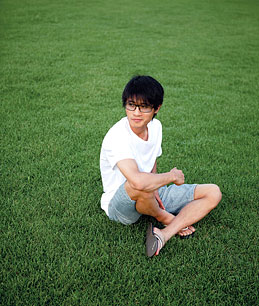
\includegraphics[scale=0.4]{han_han.jpg} 
	\end{figure}

{\tiny Photograph by Tony Law / Redux. Source: \url{http://www.time.com/time/magazine/article/0,9171,1931619,00.html}}
 \end{column}
 
 \end{columns}

\end{frame}



%%%%%%%%%%%%%%%
\begin{frame}{Background (Cont'd)}

\begin{itemize}[<+->]
\item Ghostwriting allegation against Han from January 2012
\item FANG Zhouzi 方舟子, a scientific author and anti-fraud crusader, created widespread debate on the Internet
\item {\em Light and Upright 光明与磊落}: photocopied manuscripts set, including his first novel   {\em Triple Gate 三重门} 
\item Han received a death threat on April 15, 2012
\end{itemize}

\end{frame}


%%%%%%%%%%%%%%%%
%%\section{Data}

\begin{frame}{Data Collection}
\note{


Sina Weipo provides an application programming interface (API) to access their public data.


Some technical issues: how do we access data from those website? We now have implemented a python crawler, but i believe there is a upperbound for the data you can collect within a fixed amount of time due to the weibo restriction. 
How do we design our sampling scheme? we want a way to sample data such that they can represent the whole user group of weibo. we need to know the behavior of the weibo users as some of them simply have nothing to do and posting junks all days. stratified sampling based on province? 
}

\begin{itemize}[<+->]
\item Topic searching via API: 
	\begin{itemize}
	\item Only the latest results are returned
	\item Up to 30 each time
	\end{itemize}

\item 22,398 posts collected on April 16 and 17, 2012
\item UTF-8 encoding
\end{itemize}

\end{frame}



%%%%%%%%%%%%%%%%%%%%%%%%%%%%%%%
%%%%%%%%%%%%%%%%%%%%%%%%%%%%%%%

\section{Processing}
%%%%%%

\begin{frame}{Characteristics of Chinese Language}

\begin{itemize}[<+->]
\item No explicit delimiter
\item Ambiguities in phrases
	\begin{itemize}
	\item Context ambiguition: e.g., 他好吃
	\item Word definition ambiguition: e.g., 打
	\end{itemize}
\item Out-of-vocabulary words
\item No 1-to-1 correspondence between traditional and simplified Chinese
\end{itemize}

\end{frame}


%%%%%%%%%%%%%%%%
\begin{frame}{Characteristics of Sina Weibo Posts}

 \begin{columns}[t]
 

 \begin{column}{0.6\textwidth}
 
\begin{block}{}
 \tiny
1714080953 2012-04-16 10:01:59 //@風笑巨石: 那尊神容不得别人质疑?//@伯林2011: 
质疑派人士遭到人肉,人身攻击,甚至死亡威胁的时候,从来没有污名化整个挺韩派,也没有引起什么媒体关注,相比之下,韩寒如此炒作,太无良了,挺韩和批韩的双方本不至于如此撕裂
\end{block}

\vspace{-12pt}
\begin{figure}
	  \centering
	  
\includegraphics[scale=0.35]{weiboEg.png} 
	\end{figure}
	
	
 \end{column}
 

  \begin{column}{0.4\textwidth}
	\begin{itemize}[<+->]
		\item Multiple forms
		\item Informal and short
		\item Reposting: ``$//@$''
		\item Spams
		\item Emotion symbols 
		\item Internet slangs
		\item Topic: ``\#话题\#''
	\end{itemize}
 \end{column}
 
 \end{columns}




\end{frame}

%%%%%%%%%%%%%%%
\begin{frame}[fragile]{Pre-Tagging Processing}

\begin{block}{}
1165303315 2012-04-16 09:55:40  《韩寒收到网友死亡威胁》 (来自 @新浪娱乐) http://t.cn/zOprKap
1165303315 2012-04-16 09:55:40  《Han Han received death threat online》 (from @新浪娱乐) http://t.cn/zOprKap
\end{block}


\begin{itemize}[<+->]
\item Remove user identification number and time stamp
\item Only the reposting user's comment is kept:\\
If the resulting string is empty, it will be eliminated as well
\item Remove URLs 
\item Remove duplicates 
\item 13,070 posts left
\end{itemize}


\end{frame}


%%%%%%%%%%%%%%%%
\begin{frame}{Tagging}

\begin{itemize}[<+->]
\item  Process: tagged 3000 total posts with four categories
\item Examples:
	\begin{description}
	\item[Positive] 支持韩寒! Support Han Han!
	\item[Negative] 看到韩寒就恶心。 Feel nauseous when I see Han Han.
	\end{description}


\item Limitations:
	
	\begin{itemize}
	\item Subjective responses:\\
		\quad e.g., ``that wasn't too bad''
	\item 	Uncertain tags
		\begin{itemize}
		\item Quotes
		\item Posts without subjects
		\item Posts that just mention opposing author
		\end{itemize}
	\end{itemize}

\end{itemize}

\end{frame}

%%%%%%%%%%%%%%%
\begin{frame}{Pre-Segmentation Processing}

\begin{itemize}[<+->]
\item Word segmentation is crucial for our word-based analysis
\item Substitute mentioning of topic-related usernames by the corresponding proper nouns
\item Remove other mentioned usernames
\item Substitute emotional symbols and Internet slangs  by the corresponding word surrounded by square brackets
\end{itemize}

\end{frame}


%%%%%%%%%%%%%%%%
\begin{frame}{Segmentation}

\begin{itemize}[<+->]
\item  汉语词法分析系统ICTCLAS (Institute of Computing Technology, Chinese Lexical Analysis System) is a well known Chinese word segmentation system 
\item Chinese word segmentation, lexical tagging, named entity recognition, unknown words detection, and the user-defined dictionary
\item Examples from the user-defined dictionary:
\begin{description}
\item[围脖] (wei2 bo2, means ``scarf'') refers to 微博 (Weibo, wei1 bo2)
\item[韩少] (韩: Han Han's surname, 少: abbreviation of 少爷, which means ``young master of the house'') refers to Han Han
\end{description}

\end{itemize}

\end{frame}

%%%%%%%%%%%%%%%
\begin{frame}{Conjunction Rules}
[Lee and Renganathan, 2011] suggested that special consideration should be given to
% contrasting transitional expressions
\begin{block}{}
\begin{enumerate}
\item Although (part A), (part B).
\item (Part A), but (part B).
\item Although (part A), but (part B).
\end{enumerate}
\end{block}
For each case, only part B will be kept.
\end{frame}

%%%%%%%%%%%%%%%
\begin{frame}{Stop Words and Punctuation Elimination}

\begin{itemize}[<+->]
\item Remove prepositions, punctuation marks, English character strings, interjections, modal particles, onomatopoeia, and auxiliary words
\item Remove pre-defined stop words and number strings
\end{itemize}

\end{frame}



%%%%%%%%%%%%%%%%%%%%%%%%%%%%%%%
%%%%%%%%%%%%%%%%%%%%%%%%%%%%%%%
\section{EDA}


%%%%%%%%%%%%%%%
\begin{frame}{Word Frequency}
\begin{itemize}[<+->]
\item Extract the word frequency vector $x_i$ from the $i$-th post
\item Focus on words with overall frequency $\geq$ 10, resulting in $p=795$ words
\item Construct the word frequency matrix $X=(x_1,...,x_n)^T$, where $n=3000$. This will be our design matrix.
\end{itemize}
\end{frame}
%%%%%%%%%%%%%%%%%%%%


\begin{frame}{Word Frequency Visualization: Matrix Plot}

\begin{figure}
  \centering
  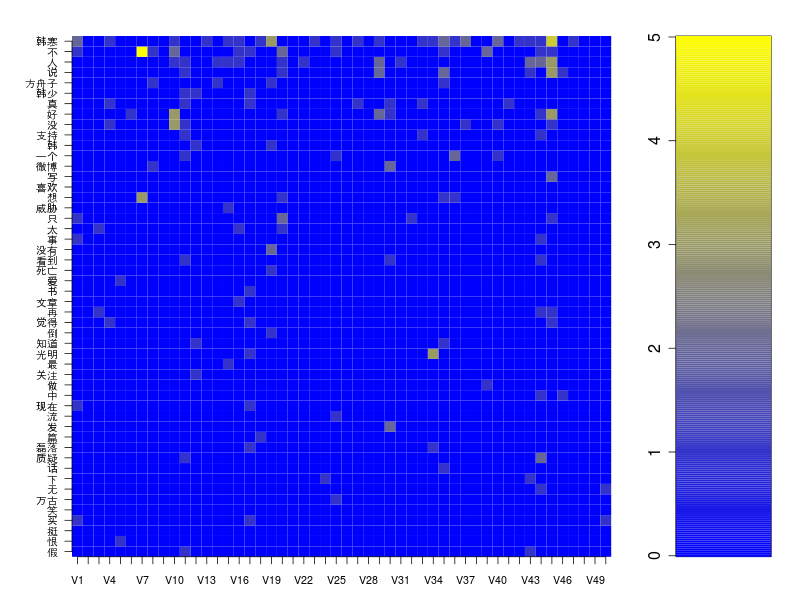
\includegraphics[height=0.9\textheight]{./../../wordFreqMat.png} 
\end{figure}
\center matrix plot of word frequency $X^T$

\end{frame}

%%%%%%%%%%%%%%%
\begin{frame}{Co-Occurrance}

\begin{figure}
  \centering
  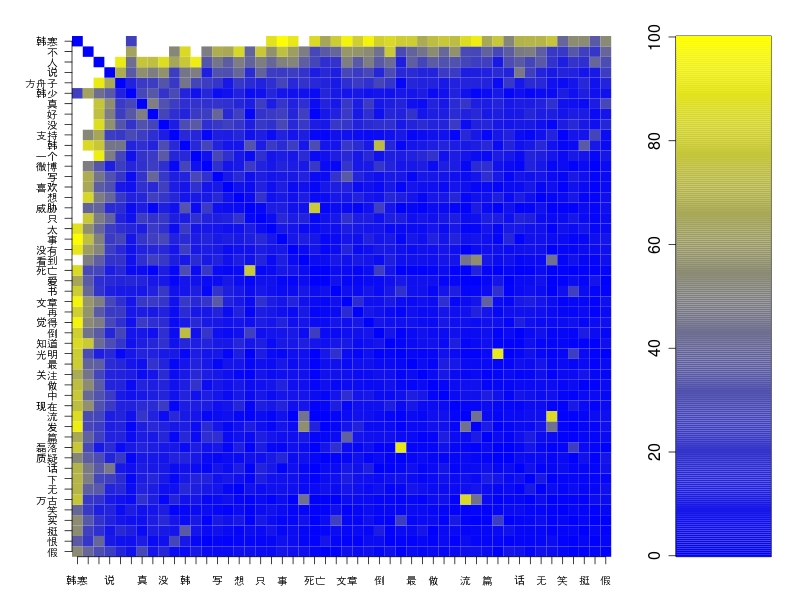
\includegraphics[height=0.9\textheight]{./../../coocurResults/cooccurMatPlot.png} 
\end{figure}


\end{frame}

%%%%%%%%%%%%%%%
\begin{frame}{Co-Occurrance}

\begin{figure}
  \centering
  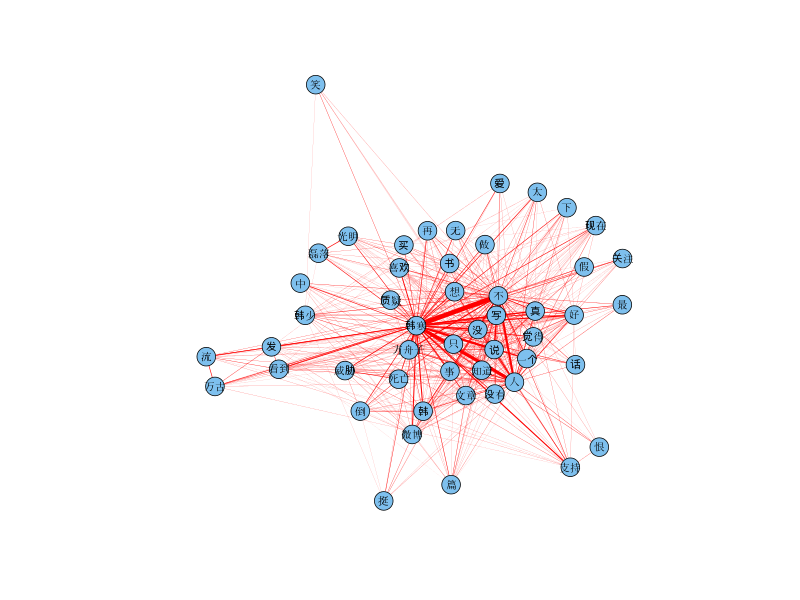
\includegraphics[height=0.9\textheight]{./../../coocurResults/cooccurNetwork.png} 
\end{figure}

\end{frame}

%%%%%%%%%%%%%%%
\begin{frame}[fragile]{Sparse Graphical Models}

\begin{itemize}[<+->]
\item Goal: study the relation between words by graphical models
\item Fact: if $x\in R^p$ follows $N(\mu,\Sigma)$, then for $i\ne j$
\begin{align*}
(x_i  \upmodels % mnsymbol
x_j )\mid \{x_{\text{all but $(i,j)$}}\} \textbf{ iff } (\Sigma^{-1})_{ij}=0
\end{align*}
\item This motivates us to estimate $\Sigma^{-1}$.
\item Let $x_1,x_2,...x_n$ be IID $N(\mu,\Sigma)$ data. The joint likelihood of the data is
\begin{align*}
& f(x_1, \dots, x_n|\mu,\Sigma) 
\\&= \frac{1}{(2\pi \det\lp \Sigma\rp)^{n/2}}\exp\left\{ -\frac{1}{2} \sum_{i=1}^n(x_i-\mu)^T\Sigma^{-1}(x_i-\mu) \right\}.
\end{align*}

\end{itemize}

\end{frame}


%%%%%%%%%%%%%%%%
\begin{frame}[fragile]{Sparse Graphical Models (Cont'd)}

\begin{itemize}[<+->]
\item  Log-likelihood:
\begin{align*}
l(\mu,\Sigma^{-1}) = -\frac{n}{2}\log \det \lp \Sigma \rp  -\frac{1}{2} \sum_{i=1}^n(x_i-\mu)^T\Sigma^{-1}(x_i-\mu)
\end{align*}

\item Do a maximum likelihood estimation (optimize over $\mu$ and $S = \Sigma^{-1}$; easy to see that the MLE for $\mu$ is $\bar{x}$):

\begin{align*}
\max_S\left\{  \frac{n}{2}\log \det\lp S \rp  -\frac{1}{2} \sum_{i=1}^n(x_i-\bar{x})^T S (x_i-\bar{x})\right\} 
\end{align*}


\end{itemize}

\end{frame}

%%%%%%%%%%%%%%%
\begin{frame}[fragile]{Sparse Graphical Models (Cont'd)}

\begin{itemize}[<+->]
\item  Trace trick $\sum_{i=1}^n(x_i-\bar{x})^T S (x_i-\bar{x}) = \textbf{Tr} (\sum_{i=1}^n (x_i-\bar{x})(x_i-\bar{x})^TS) = n\textbf{Tr}(\hat{\Sigma}S)$. We end up with:
\begin{align*}
\max_S \left\{  \log \det \lp S\rp - \textbf{Tr}(\hat{\Sigma}S )  \right\}
\end{align*}

\item  Fitting a sparse Gaussian graphical model:
\begin{align*}
\max_S \left\{ \log \det S - \textbf{Tr} ( \hat{\Sigma}S ) - \lambda ||S||_1 \right\}
\end{align*}
where $||S||_1 = \sum_{i,j}|s_{ij}|$. See, e.g. Banerjee et al. (2007) and Friedman et al. (2007). 

\end{itemize}

\end{frame}

%%%%%%%%%%%%%%%%
\begin{frame}{Sparse Graphical Models: Results}

\begin{figure}
  \centering
  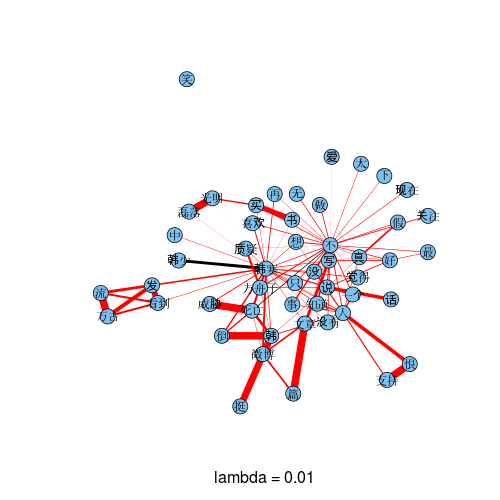
\includegraphics[height=0.9\textheight]{./../../gLassoResults/glasso1.png} 
\end{figure}
\center Top 50 words usage network
\end{frame}

%%%%%%%%%%%%%%%
\begin{frame}{Sparse Graphical Models: Results}

\begin{figure}
  \centering
  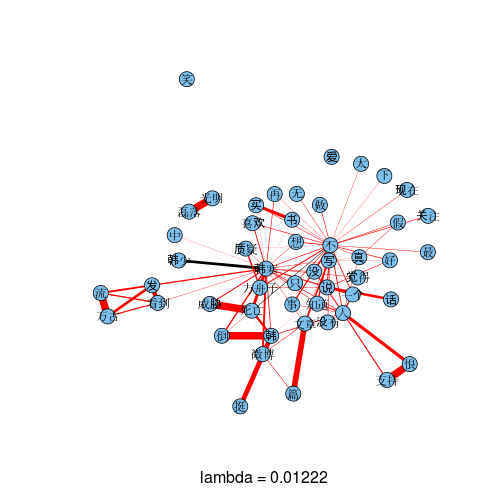
\includegraphics[height=0.9\textheight]{./../../gLassoResults/glasso2.png} 
\end{figure}
\center Top 50 words usage network

\end{frame}
%%%%%%%%%%%%%%%
\begin{frame}{Sparse Graphical Models: Results}

\begin{figure}
  \centering
  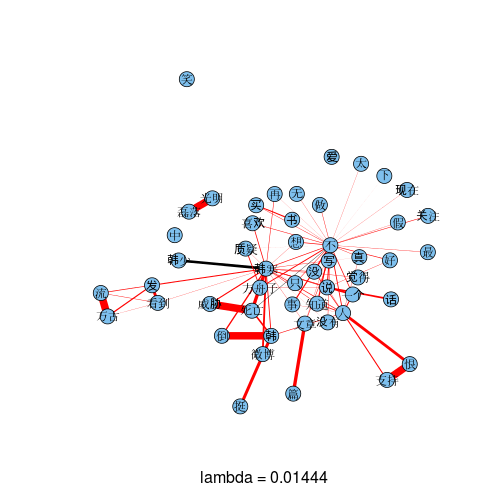
\includegraphics[height=0.9\textheight]{./../../gLassoResults/glasso3.png} 
\end{figure}
\center Top 50 words usage network

\end{frame}
%%%%%%%%%%%%%%%
\begin{frame}{Sparse Graphical Models: Results}

\begin{figure}
  \centering
  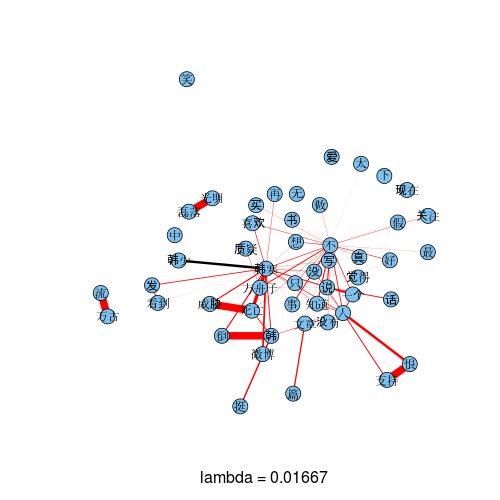
\includegraphics[height=0.9\textheight]{./../../gLassoResults/glasso4.png} 
\end{figure}
\center Top 50 words usage network

\end{frame}
%%%%%%%%%%%%%%%
\begin{frame}{Sparse Graphical Models: Results}

\begin{figure}
  \centering
  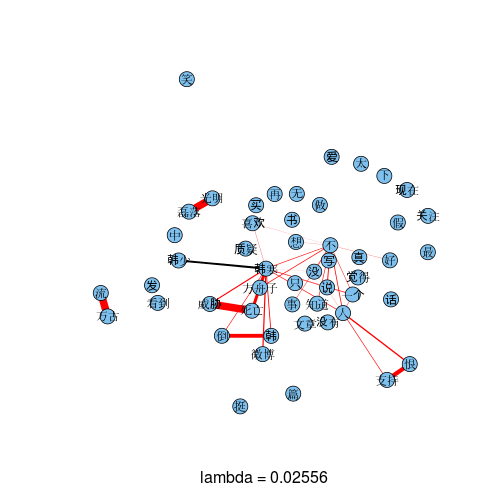
\includegraphics[height=0.9\textheight]{./../../gLassoResults/glasso5.png} 
\end{figure}
\center Top 50 words usage network

\end{frame}
%%%%%%%%%%%%%%%
\begin{frame}{Sparse Graphical Models: Results}

\begin{figure}
  \centering
  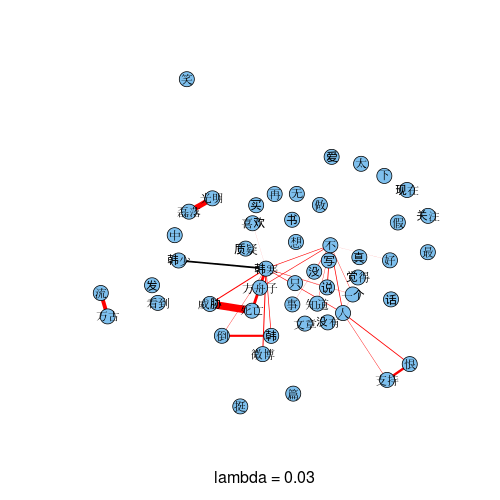
\includegraphics[height=0.9\textheight]{./../../gLassoResults/glasso6.png} 
\end{figure}
\center Top 50 words usage network

\end{frame}

%%%%%%%%%%%%%%%%
\begin{frame}{Sparse Graphical Models v.s. Co-Occurence}

\begin{figure}
  \centering
  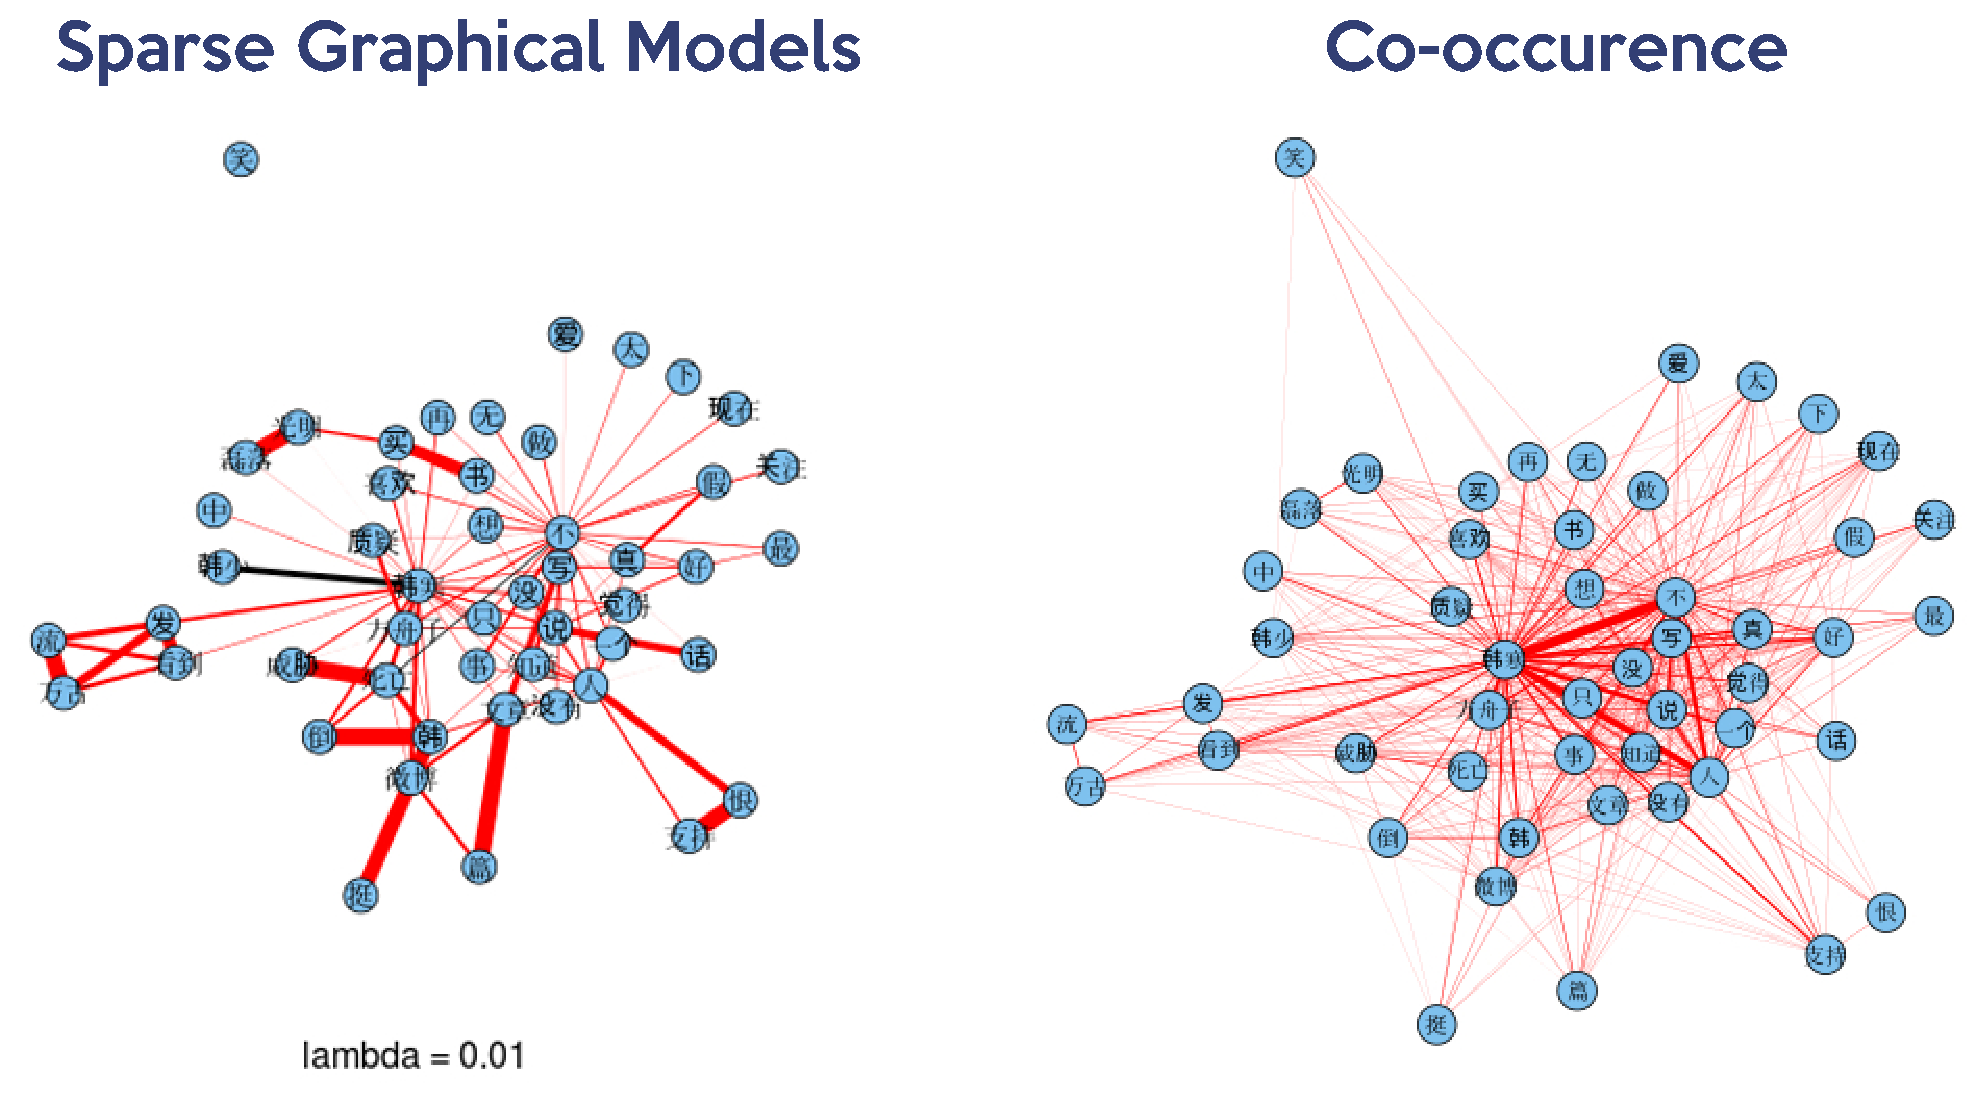
\includegraphics[scale=0.35]{sgmVScooc.pdf} 
\end{figure}

\end{frame}

\clearpage 
%%%%%%%%%%%%%%%%%%%%%%%%%%%%%%
%%%%%%%%%%%%%%%%%%%%%%%%%%%%%%
\section{Classification}

\begin{frame}{Classification}

\note{ I will talk about this slide and Christine continues the next}

\begin{itemize}[<+->]


\item $x_i\in R^{p}$ be the $i$-th row of $X\in R^{n\times p}$, where $n=3000$ and $p=395$
\item $y_i$: the corresponding category. Assume $y_i\in\{-1,+1\}$, where the $+1$ can have one (and only one) of the following meanings (at a time):
  \begin{itemize}[<+->]
    \item positive feeling about Han Han
    \item negative feeling about Han Han 
    \item netural or unidentifiable opinion 
    \item spam
\end{itemize}
\item Two classification methods: LASSO and $l_1$-norm SVM.
\end{itemize}
\end{frame}
%%%%%%%%%%%%%%%
\subsection{LASSO}

%%%
\begin{frame}[fragile]{LASSO}
\begin{itemize}[<+->]

\item The Lasso approach (Tibshirani, (1996)):
\[
\hat{\beta}(\lambda) = \arg \min_\beta \frac{1}{2}||y-(\beta_0+X\beta)||_2^2 + \lambda ||\beta||_1
\]
\item The classifier:
\[
\text{class}(x) = \textbf{sign}(\beta_0+x^T\beta)\in\{-1,+1\}
\]

\item Four models for each category for classification
\item General overview of method
\item General overview of application to data
	\begin{itemize}
	\item for 4 categories
	\item 10 fold CV
	%\item Frequency matrix is $3000 \times 795$
	\item classification error
	\end{itemize}
	
\end{itemize}

\end{frame}

%%%%%%%%%%%%%%%%
\begin{frame}{Choosing $\lambda$: Cross-Validation}

\begin{figure}
  \centering
  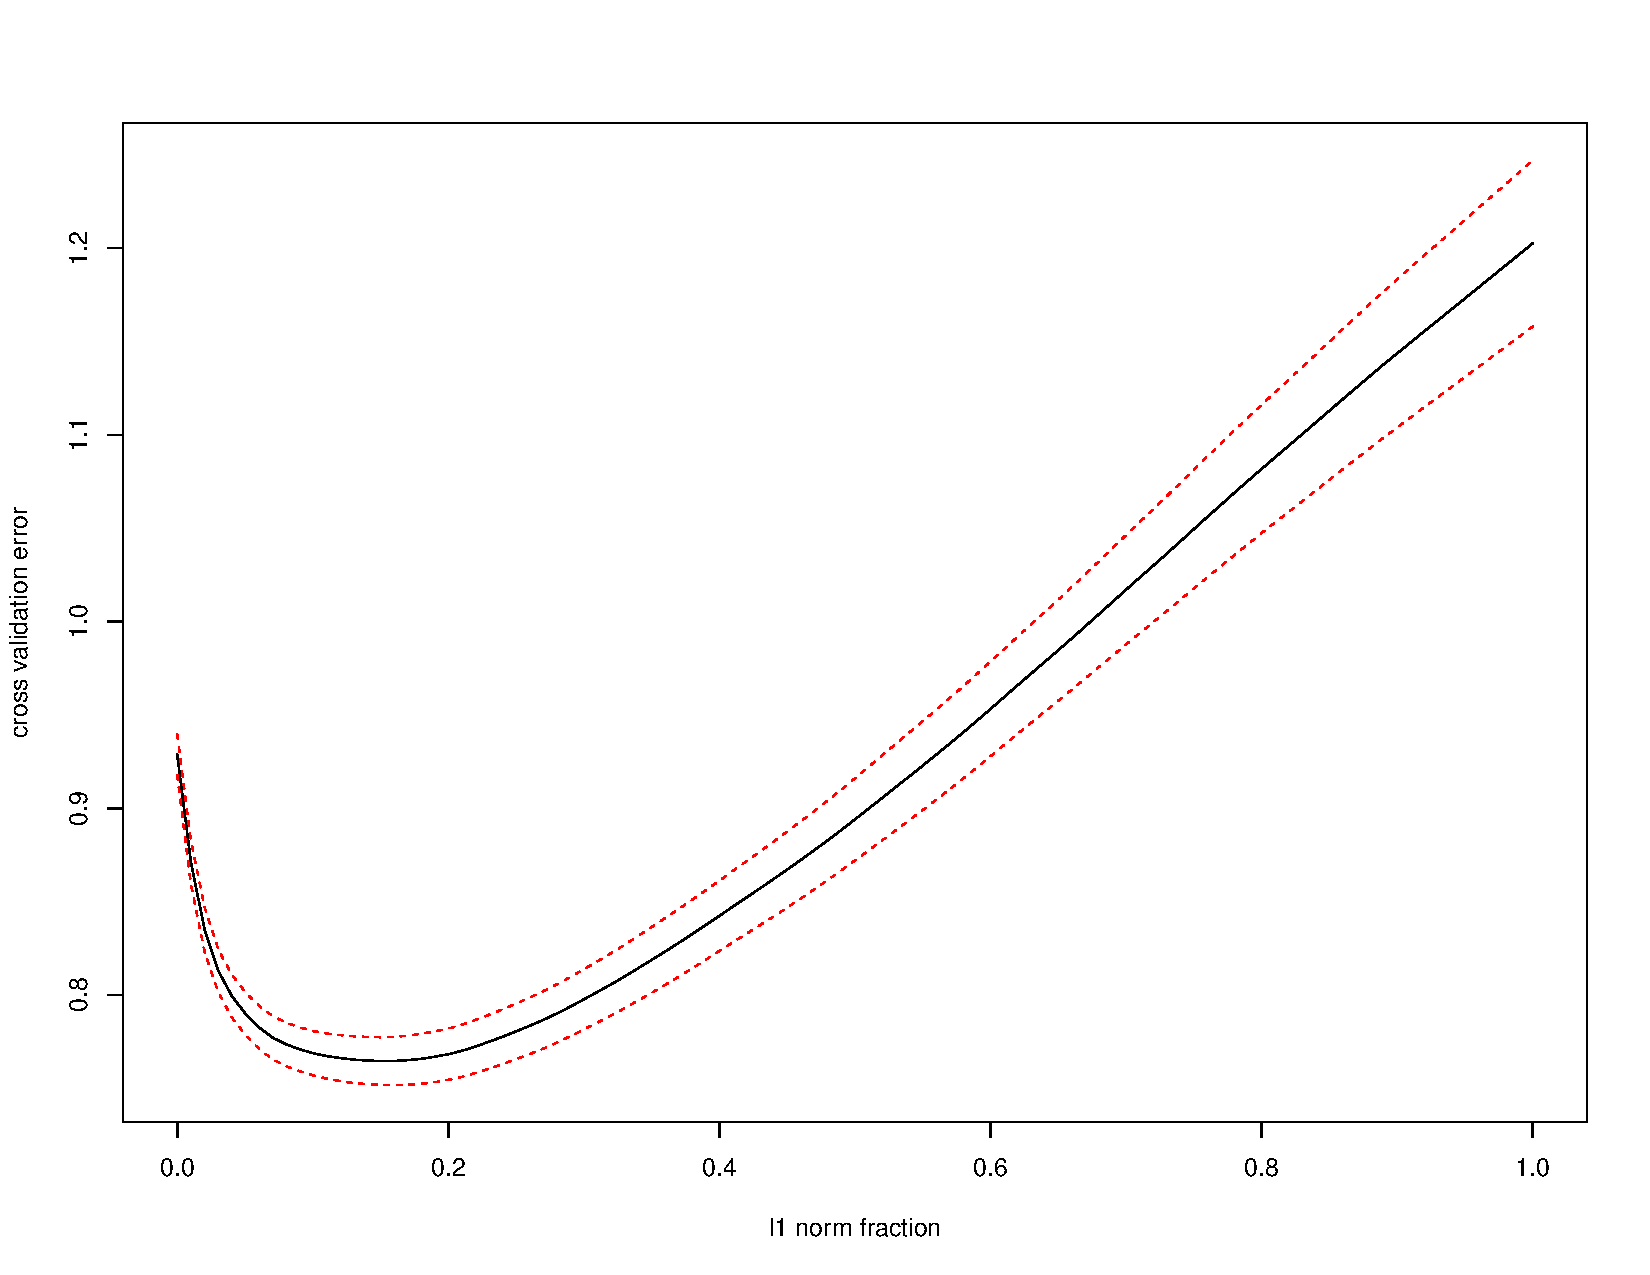
\includegraphics[height=0.9\textheight]{./../../lassoResults/CVPosErr.pdf} 
\end{figure}

\end{frame}


%%%
\begin{frame}{LASSO Coefficient interpretation} 

\begin{itemize}[<+->]
\item The classifier:
\[
\text{class}(x) = \textbf{sign}(\beta_0+x^T\beta)\in\{-1,+1\}
\]
\item We can look at coefficients $\beta$

	\begin{itemize}
	\item Absolute value: most relevant/predictive words
	\item Positive: more likely to classify the post in $+1$ category (all other covariates being fixed)
	\item Negative: more likely to be in $-1$ category	
	\end{itemize}
	
\end{itemize}

\end{frame}



%%%%%%%%%%%%%%%
\begin{frame}{Positive v.s. Nonpositive Classification Result}

\begin{itemize}[<+->]
\item $y_i\in\{-1,+1\}$;
\item $+1$: positive opinion (about Han Han);
\item $-1$: non-positive opinion, including negative, neutral and spam.
\end{itemize}

\tiny
\begin{center}
\begin{tabular}{|c|c||c|c||c|c|}
\hline
Word & Absolute Coef. & Word & Positive Coef. & Word & Negative Coef.\\ \hline \hline
加油 & 0.820 & 加油 & 0.820 & 样子 & -0.396\\
(keep going) & & (keep going) & & (manner) & \\\hline
韩少 & 0.644 & 韩少 & 0.644 & 恋 & -0.344\\
(Master Han) & & (Master Han) & & (love) & \\\hline
成熟 & 0.546 & 成熟 & 0.546 & 发表 & -0.336\\
(mature) & & (mature) & & (announce) & \\\hline
顶 & 0.533 & 顶 & 0.533 & 道理 & -0.336\\
(support) & & (support) & & (rational) & \\\hline
宽容 & 0.518 & 宽容 & 0.518 & 利益 & -0.335\\
(tolerant) & & (tolerant) & & (benefit) & \\\hline
\end{tabular}
LASSO word images for the positive v.s. nonpositive classification.
\end{center}


\end{frame}


%%%%%%%%%%%%%%%%
\begin{frame}{Negative v.s. Nonnegative Classification Result}
\note{
(To Angie: please delete the zero entries)
(To Christine: remember to talk about why there are four empty entries; this is probably due to the size of nega sample is too small)
}
\begin{itemize}[<+->]
\item $+1$: negative opinion;
\item $-1$: non-negative opinion, including positive, neutral and spam.
\end{itemize}

\tiny
\begin{center}
\begin{tabular}{|c|c||c|c||c|c|}
\hline
Word & Absolute Coef. & Word & Positive Coef. & Word & Negative Coef.\\ \hline \hline
讨厌 & 0.481 & 讨厌 & 0.481 & 支持 & -0.008\\
(hate) & & (hate) & & (support) & \\\hline
无耻 & 0.412 & 无耻 & 0.412 &  & -\\
(shameless) & & (shameless) & & - & \\\hline
恶心 & 0.395 & 恶心 & 0.395 &  & -\\
(disgusting) & & (disgusting) & & - & \\\hline
骗子 & 0.380 & 骗子 & 0.380 &  & -\\
(liar) & & (liar) & & - & \\\hline
扁 & 0.353 & 扁 & 0.353 & - & -\\
(beat up) & & (beat up) &- & - & \\\hline
\end{tabular}
LASSO word images for the negative v.s. nonnegative classification.
\end{center}

\end{frame}


%%%%%%%%%%%%%%%%
%%\begin{frame}{LASSO: Negative}
%%
%%\begin{figure}
%%  \centering
%%  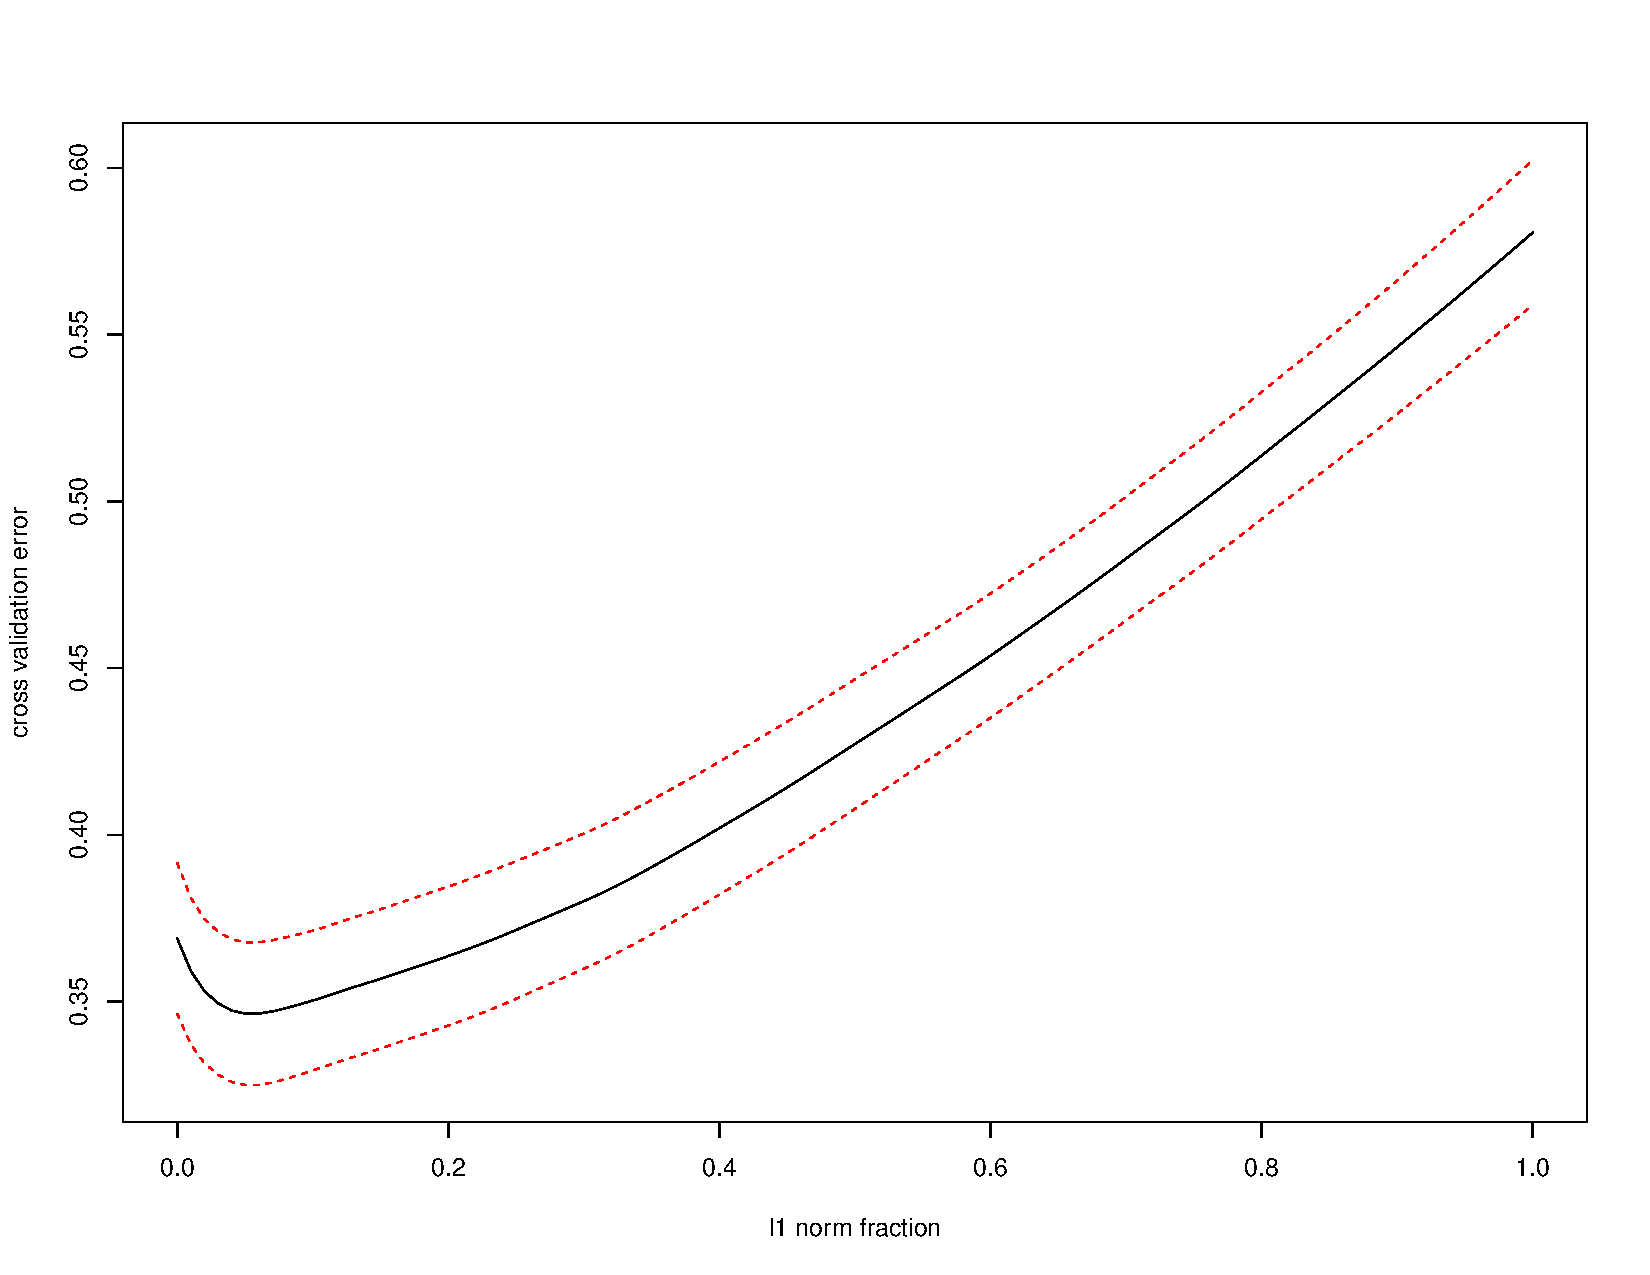
\includegraphics[height=0.9\textheight]{./../../lassoResults/CVNegErr.pdf} 
%%\end{figure}
%%
%%\end{frame}
%%
%%%%%%%%%%%%%%%%%
%%\begin{frame}{LASSO: Neutral}
%%
%%\begin{figure}
%%  \centering
%%  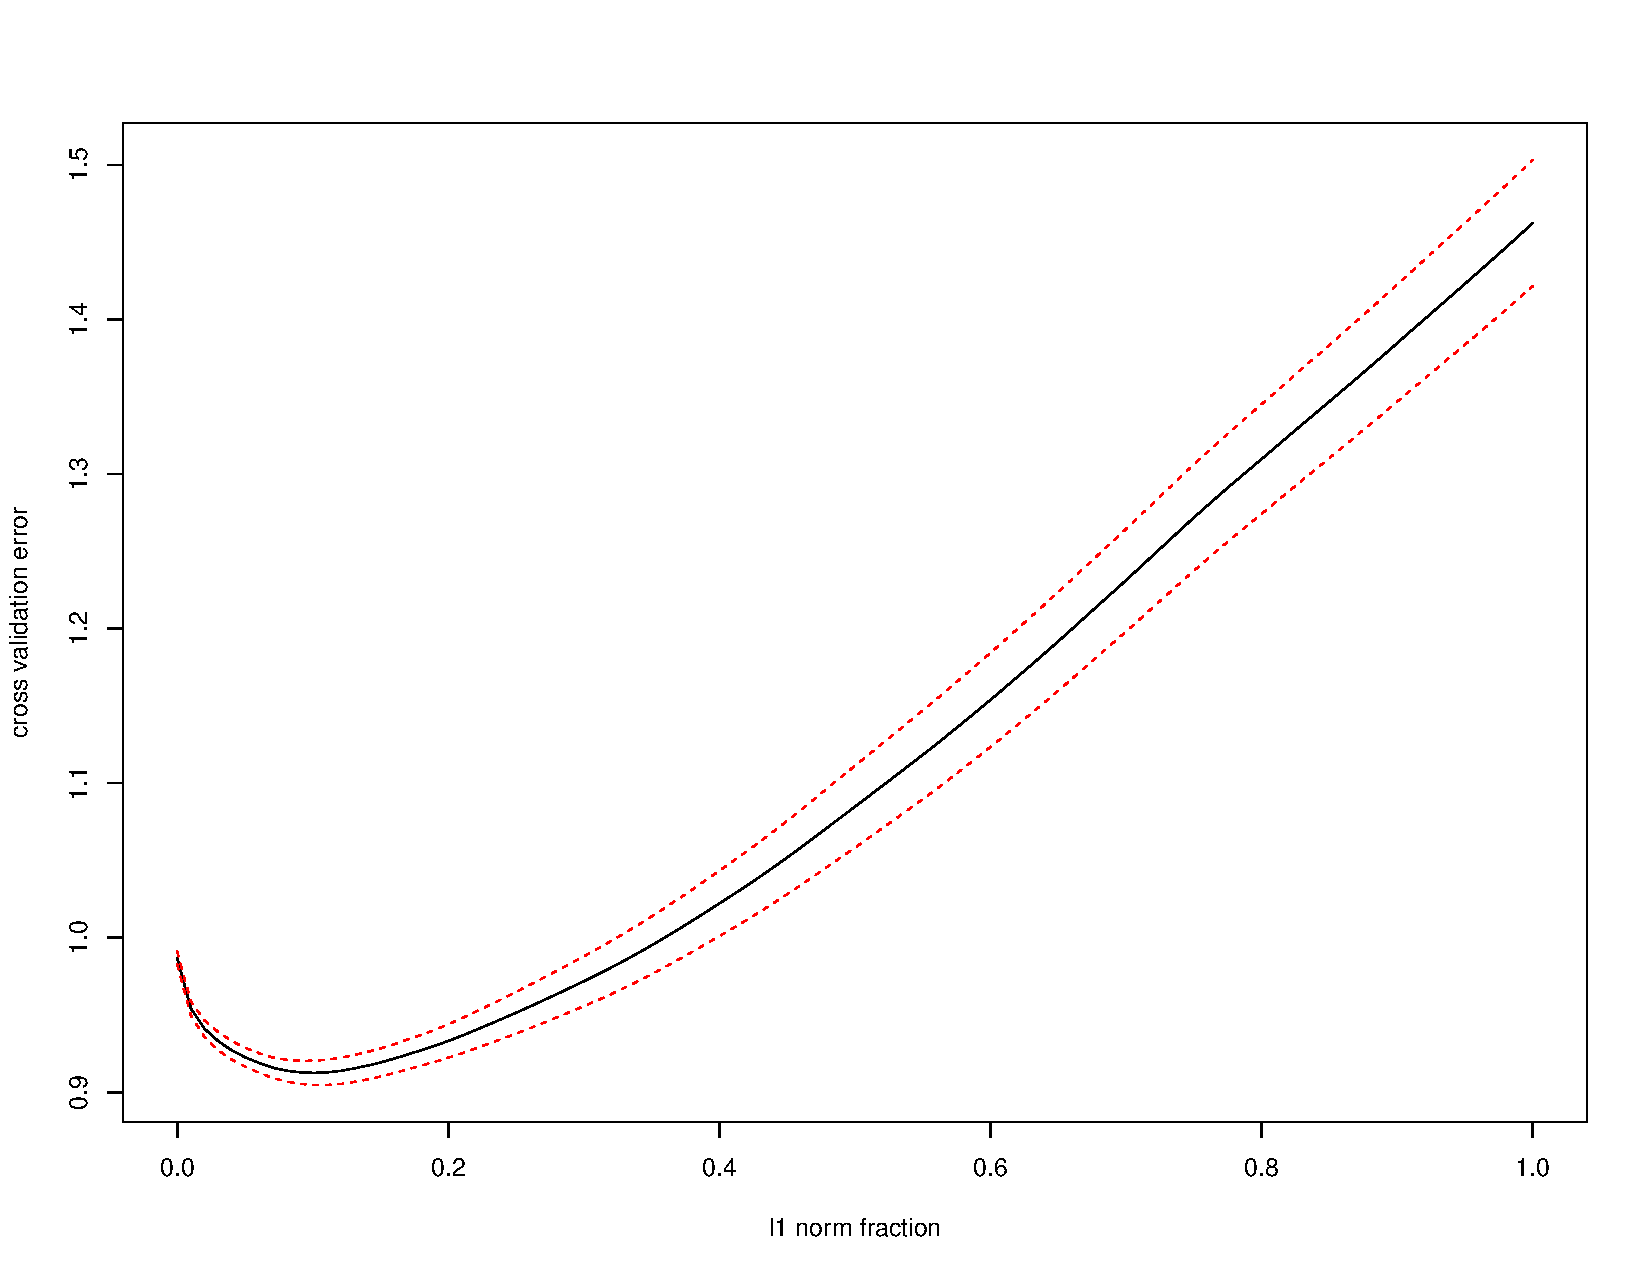
\includegraphics[height=0.9\textheight]{./../../lassoResults/CVNeuErr.pdf} 
%%\end{figure}
%%
%%\end{frame}
%%
%%%%%%%%%%%%%%%%%
%%\begin{frame}{LASSO: Spam}
%%
%%\begin{figure}
%%  \centering
%%  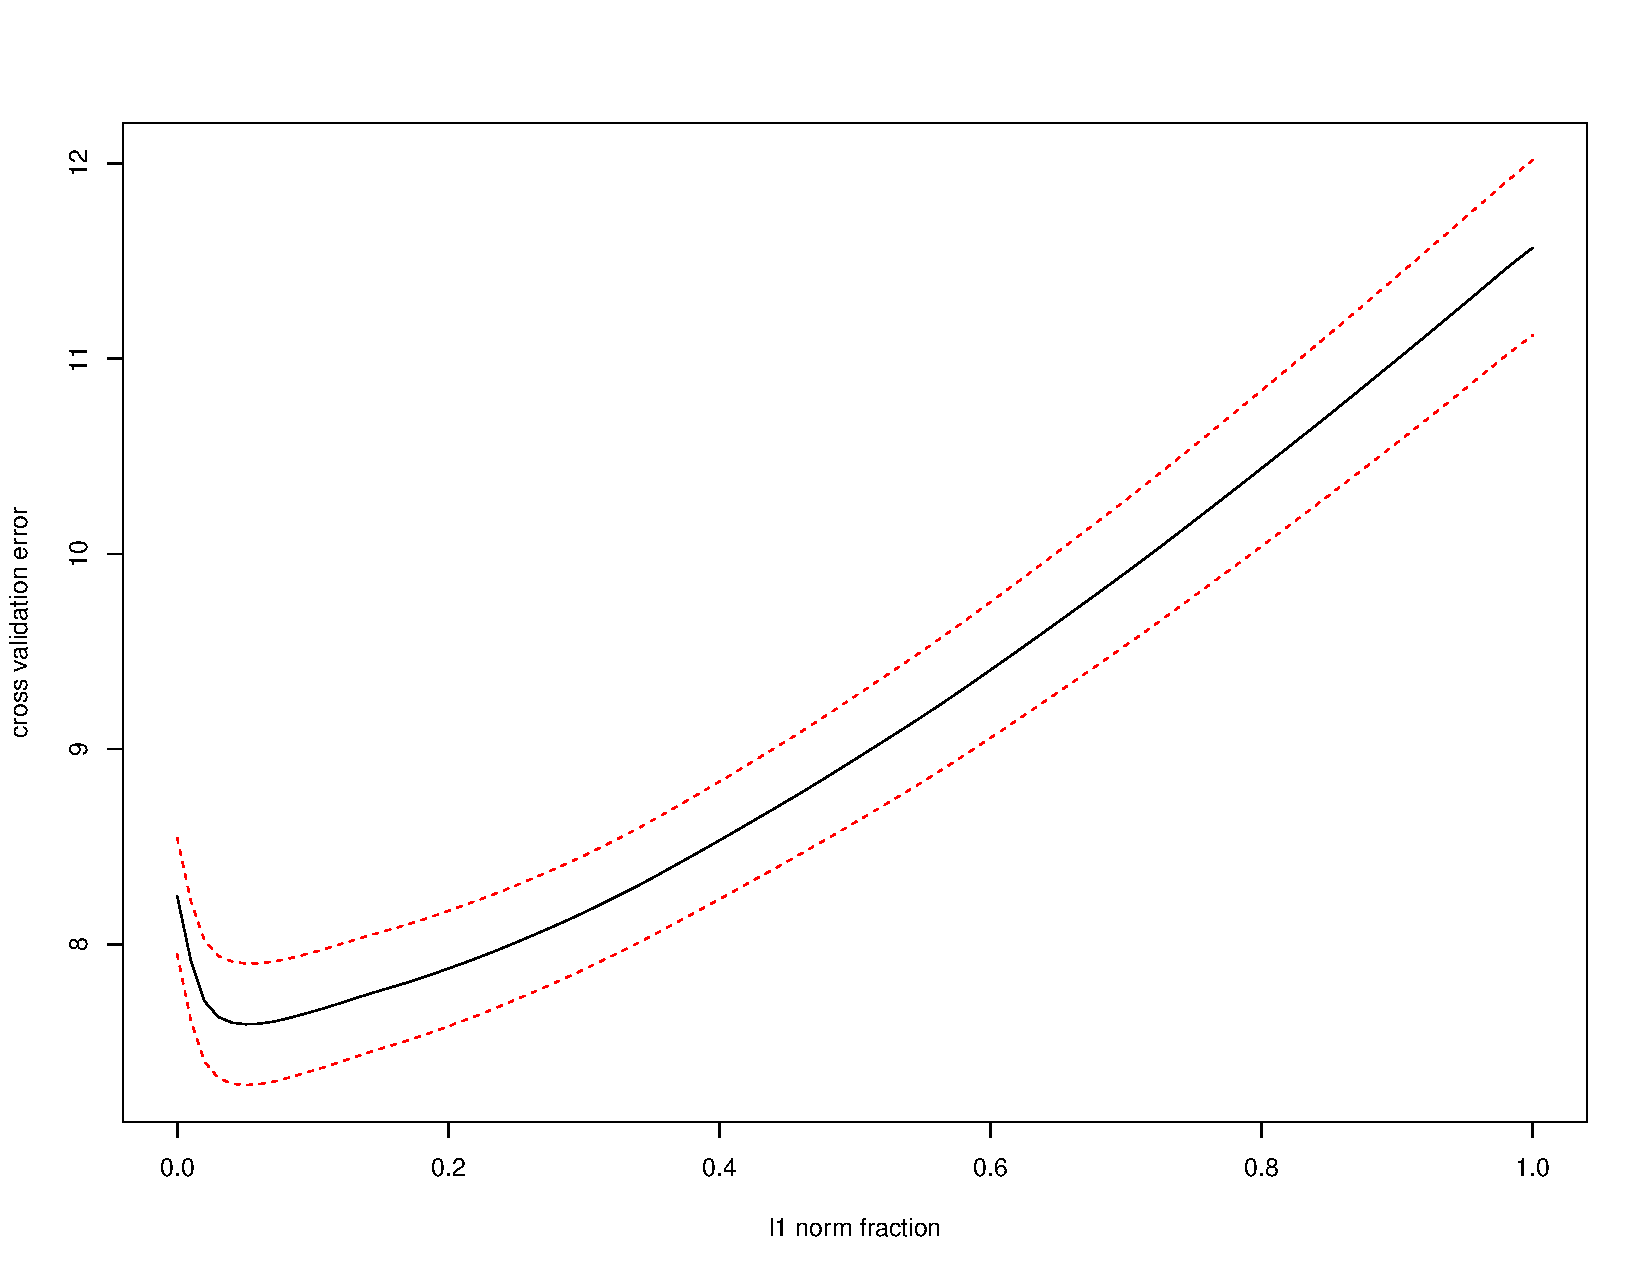
\includegraphics[height=0.9\textheight]{./../../lassoResults/CVSpamErr.pdf} 
%%\end{figure}
%%
%%\end{frame}
%%
%%%%%%%%%%%%%%%%

\subsection{$l_1$-Norm Support Vector Machine}
%%%%%%%%%%%%%%%
\begin{frame}[fragile]{Standard Support Vector Machine}

\begin{itemize}[<+->]
\item Again, linear decision function $f(x) = \beta_0 + \beta x$;
\item The classifier $\text{class}(x) = \textbf{sign} (f(x))$. 
\item  The support vector machine (SVM) (see, e.g. Hastie et al 2001): 
\begin{align*}
\min_{\beta_0,\beta} \sum_{i=1}^n(1-y_if(x_i))_+ + \frac{\lambda}{2} ||\beta||_2^2,
\end{align*}
where $z_+ = \max(0,z)$. 
\end{itemize}

\end{frame}


%%%%%%%%%%%%%%%
\begin{frame}[fragile]{$l_1$-Norm Support Vector Machine}

\begin{itemize}[<+->]  
\item Replacing the $l_2$-norm by $l_1$-norm yields the sparse SVM (Zhu et al 2003):
\begin{align*}
\min_{\beta_0,\beta} \left\{ \sum_{i=1}^n(1-y_if(x_i))_+ + \lambda ||\beta||_1\right\}. 
\end{align*}
\item Computation: use the matlab \textbf{lpsvm} package by Fung and Mangasarian (2002)
\end{itemize}

\end{frame}


%%%%%%%%%%%%%%%%%%%%%%%%%%%%%%
%%%%%%%%%%%%%%%
\begin{frame}{Positive v.s. Nonpositive Classification Result}

\begin{itemize}[<+->]
\item $+1$: positive opinion;
\item $-1$: non-positive opinion, including negative, neutral and spam.
\item Cross validation result: 
  \begin{itemize}[<+->]
  \item training sample misclassification rate: 16.9\%
  \item testing sample misclassification rate: 28.2\%
  \end{itemize}

\end{itemize}

%\end{frame}

%\begin{frame}{Positive v.s. Nonpositive Classification Result}
\tiny
% put the table here
\begin{tabular}{|c|c||c|c||c|c|}
\hline
Word & Absolute Coef. & Word & Positive Coef. & Word & Negative Coef.\\ \hline \hline
加油 & 2.340 & 加油 & 2.340 & 铁证 & 2.305\\
(keep going) & & (keep going) & & (clear evidence) & \\\hline
铁证 & 2.305 & 家人 & 2.269 & 接受 & 2.061\\
(clear evidence) & & (family) & & (accept) & \\\hline
家人 & 2.269 & 韩少 & 1.969 & 媒体 & 1.907\\
(family) & & (Master Han) & & (media) & \\\hline
接受 & 2.061 & 成熟 & 1.806 & 默默 & 1.883\\
(accept) & & (mature) & & (quietly) & \\\hline
韩少 & 1.969 & 顶 & 1.803 & 四娘 & 1.762\\
(Master Han) & & (support) & & (GUO Jingming) & \\\hline
\end{tabular}
\begin{center} 
$l_1$-SVM word images for the positive v.s. positive classification.
\end{center}

\end{frame}

%%%%%%%%%%%%%%%%%%%%%%%%
%%%%%%%%%%%%%%%
\begin{frame}{Negative v.s. Nonnegative Classification Result}
\footnotesize
\begin{itemize}[<+->]
\item $+1$: negative opinion;
\item $-1$: non-negative opinion, including positive, neutral and spam.
\item Cross validation result: 
  \begin{itemize}[<+->]
  \item training sample misclassification rate: 6.4\%
  \item testing sample misclassification rate: 11.5\%
  \end{itemize}

\end{itemize}


\vspace{-3pt}
%put the table here
\tiny
\begin{tabular}{|c|c||c|c||c|c|}
\hline
Word & Absolute Coef. & Word & Positive Coef. & Word & Negative Coef.\\ \hline  \hline
扁 & 1.777 & 扁 & 1.777 & 脑子 & 1.447\\
(beat up) & & (beat up) & & (mind) & \\\hline
苦肉计 & 1.708 & 苦肉计 & 1.708 & 彻底 & 1.290\\
(the use of  & & (the use of  &  &  (completely) &  \\
self-injury to win & &  self-injury to win &  & &  \\
somebody's & & somebody's  &  & &  \\
 confidence) & &  confidence)  &  & &  \\\hline
恶心 & 1.527 & 恶心 & 1.527 & 送给 & 1.221\\
(disgusting) & & (disgusting) & & (give) & \\\hline
脑子 & 1.447 & 骗子 & 1.301 & 感觉 & 1.109\\
(asdf) & & (liar) & & (feel) & \\\hline
骗子 & 1.301 & 公开 & 1.220 & 热点 & 1.101\\
(liar) & & (open) & & (hot interest) & \\\hline
\end{tabular}
\begin{center}
$l_1$-SVM word images for the negative v.s. nonnegative classification.
\end{center}

\end{frame}

%%%%%%%%%%%%%%%
\begin{frame}{$l_1$-Norm SVM v.s. LASSO}

\begin{center}
Positive v.s. Nonpositive Classification Results

Positive coefficients
\end{center}

\footnotesize
\begin{center}
\begin{tabular}{|c|c||c|c|}
\hline
$l_1$-Norm SVM & & LASSO &  \\ \hline
Word & Postive Coef. & Word & Positive Coef.\\ \hline\hline
加油 & 2.340 & 加油 & 0.820\\
(keep going) & & (keep going) &\\\hline
家人 & 2.269 & 韩少 & 0.644\\
(family) & & (Master Han) &  \\\hline
韩少 & 1.969 & 成熟 & 0.546\\
(Master Han) & & (mature) &  \\\hline
成熟 & 1.806 & 顶 & 0.533\\
(mature) & & (support) &  \\\hline
顶 & 1.803 & 宽容 & 0.518\\
(support) & & (tolerant) &  \\\hline
\end{tabular}
\end{center}





\end{frame}

%%%%%%%%%%%%%%%%%%%%%%%%%%%%%%
\section{Further Work}

%%%%%%%%%%%%%%%
\begin{frame}{Further Work}

\begin{itemize}[<+->]
\item Comparison with maximum entropy approach
\item Graphical model to track reposting
\item Statistical models for identifying Internet slangs
\item Sampling from large graphs
\end{itemize}

\end{frame}





%%%%%%%%%%%%%%%%%%%%%%%%%%%%%%
%%%%%%%%%%%%%%%%%%%%%%%%%%%%%%
%%%%%%%%%%%%%%%
%\begin{frame}{}
%
%\begin{itemize}[<+->]
%\item  .
%\end{itemize}
%
%\end{frame}
%
%%%%%%%%%%%%%%%%
%\begin{frame}{}
%
%\begin{itemize}[<+->]
%\item  .
%\end{itemize}
%
%\end{frame}
%
%
%%%%%%%%%%%%%%%%
%\begin{frame}{}
%
%\begin{itemize}[<+->]
%\item  .
%\end{itemize}
%
%\end{frame}
%
%%%%%%%%%%%%%%%%
%\begin{frame}{}
%
%\begin{itemize}[<+->]
%\item .
%\end{itemize}
%
%\end{frame}
%
%
%%%%%%%%%%%%%%%%
%\begin{frame}{}
%
%\begin{itemize}[<+->]
%\item  .
%\end{itemize}
%
%\end{frame}
%
%%%%%%%%%%%%%%%%
%\begin{frame}{}
%
%\begin{itemize}[<+->]
%\item  .
%\end{itemize}
%
%\end{frame}
%
%%%%%%%%%%%%%%%%
%\begin{frame}{}
%
%\begin{itemize}[<+->]
%\item .
%\end{itemize}
%
%\end{frame}
%
%




\end{document}
